\documentclass[a4paper, 12pt]{article}
\usepackage[a4paper,top=1.5cm, bottom=1.5cm, left=1cm, right=1cm]{geometry}
\usepackage{cmap}					% поиск в PDF
\usepackage{mathtext} 				% русские буквы в формулах
\usepackage[T2A]{fontenc}			% кодировка
\usepackage[utf8]{inputenc}			% кодировка исходного текста
\usepackage[english,russian]{babel}	% локализация и переносы

\usepackage{amsmath,amssymb}
\usepackage{indentfirst}
\usepackage{longtable}
\usepackage{graphicx}
\usepackage{array}
\usepackage{float}

\usepackage{floatflt}
\usepackage{wrapfig}
\usepackage{siunitx} % Required for alignment
\usepackage{subfigure}
\usepackage{multirow}
\usepackage{rotating}
\usepackage{caption}

\graphicspath{{.}}


\title{\begin{center}Лабораторная работа №3.4.5\end{center}
Петля гистерезиса (динамический метод)}
\author{Рожков А. В.}
\date{\today}

\begin{document}
    \pagenumbering{gobble}
    \maketitle
    \newpage
    \pagenumbering{arabic}

    \textbf{Цель работы:} изучение петель гистерезиса различных ферромагнитных материалов в переменных токах.

    \textbf{В работе используются:} автотрансформатор, понижающий трансформатор, интегрирующая цепочка, амперметр, вольтметр, электронный осциллограф, делитель напряжения, тороидальные образцы с двумя обмотками (с сердечниками из феррита, пермаллоя и кремнистого железа).

    \section{Теоретическая справка}

        Магнитная индукция $B$ и напряжённость поля $H$ в ферромагнитном материале неоднозначно связаны между собой: индукция зависит не только от напряжённости, но и от предыстории образца. Связь между $B$ и $H$ типичного ферромагнетика иллюстрирует рисунок \ref{theor}.

        \begin{figure}[h]
            \centering
            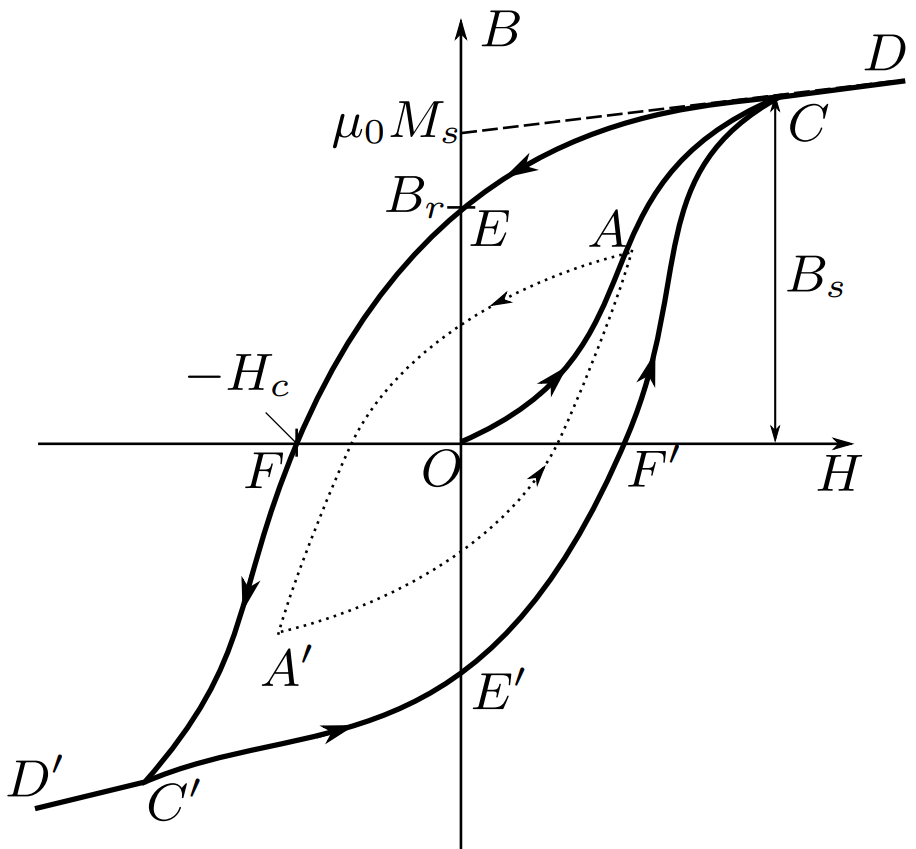
\includegraphics[scale=0.45]{img/theor.png}
            \caption{Петля гистерезиса ферромагнетика} \label{theor}
        \end{figure}

        Если к ферромагнитному образцу прикладывать переменное внешнее магнитное поле, то его состояние на плоскости $H-B$ будет изменяться по замкнутой кривой -- \textit{петле гистерезиса}. Размер петли определяется максимальным значением напряжённости $H$ в цикле (например, петля $AA'$, обозначенная пунктиром на рисунке \ref{theor}). Если амплитуда напряжённости достаточно велика, то образец будет периодически достигать \textit{насыщения}, что на рисунке соответствует кривой $CERC'E'F'C$ (\textit{предельная петля гистерезиса}). Пересечение предельной петли с вертикальной осью соответствует остаточной индукции $B_r$, пересечение с горизонтальной осью -- коэрцитивному полю $H_c$. Крайние точки петель, соответствующие амплитудным значениям $H$ (например, точка $A$ на рисунке \ref{theor}), лежат на \textit{начальной кривой намагничивания} ($OAC$).

        \textbf{Измерение магнитной индукции.} Магнитную индукцию $B$ удобно определять с помощью ЭДС, возникающей при измерении магнитного потока $\Phi$ в катушке, намотанной на образец. Пусть катушка с $N$ витками плотно охватывает образец сечением $S$, и индукция $B$ в образце однородна. Тогда\[\left|B\right|=\frac{1}{SN}\int\varepsilon\text{d}t.\]Таким образом, для определения $B$ нужно проинтегрировать сигнал, наведённый меняющимся магнитным полем в измерительной катушке, намотанной на образец.

        Для интегрирования в работе используется \textit{интегрирующая} $RC$-цепочка. Входное напряжение от источника $U_{\text{вх}}(t)$ подаётся на последовательно соединённые резистор $R_{\text{и}}$ и конденсатор $C_{\text{и}}$. Выходное напряжение $U_{\text{вых}}(t)$ снимается с конденсатора. Предположим, что (1) сопротивление источника мало по сравнению с $R_{\text{и}}$; (2) выходное сопротивление (сопротивление на входе осциллографа), напротив, велико: $R_{\text{вых}}\gg R_{\text{и}}$; и, наконец, (3) сопротивление $R_{\text{и}}$ достаточно велико, так что почти всё падение напряжения приходится на него, а $U_{\text{вых}}\ll U_{\text{вх}}$. В таком случае ток цепи равен $I=\frac{U_{\text{вх}}-U_{\text{вых}}}{R_{\text{и}}}\approx\frac{U_{\text{вх}}}{R_{\text{и}}}$, и входное и выходное сопротивление связаны соотношением\[U_{\text{вых}}\frac{q}{C_{\text{и}}}=\frac{1}{C_{\text{и}}}\int_0^tI\text{d}t\approx\frac{1}{\tau_{\text{и}}}\int_0^tU_{\text{вх}}\text{d}t,\]где $\tau_{\text{и}}=R_{\text{и}}C_{\text{и}}$ -- постоянная времени $RC$-цепочки. Для индукции поля получаем\[\left|B\right|=\frac{1}{SN}\int U_{\text{вх}}\text{d}t=\frac{\tau_{\text{и}}}{SN}U_{\text{вх}}.\]

    \section{Экспериментальная установка}

        Схема установки приведена на рисунке \ref{device}. Напряжение сети (220 Вт, 50 Гц) с помощью регулировочного автотрансформатора Ат через разделительный понижающий трансформатор Тр подаётся на намагничивающую обмотку $N_0$ исследуемого образца.

        \begin{figure}[h]
            \centering
            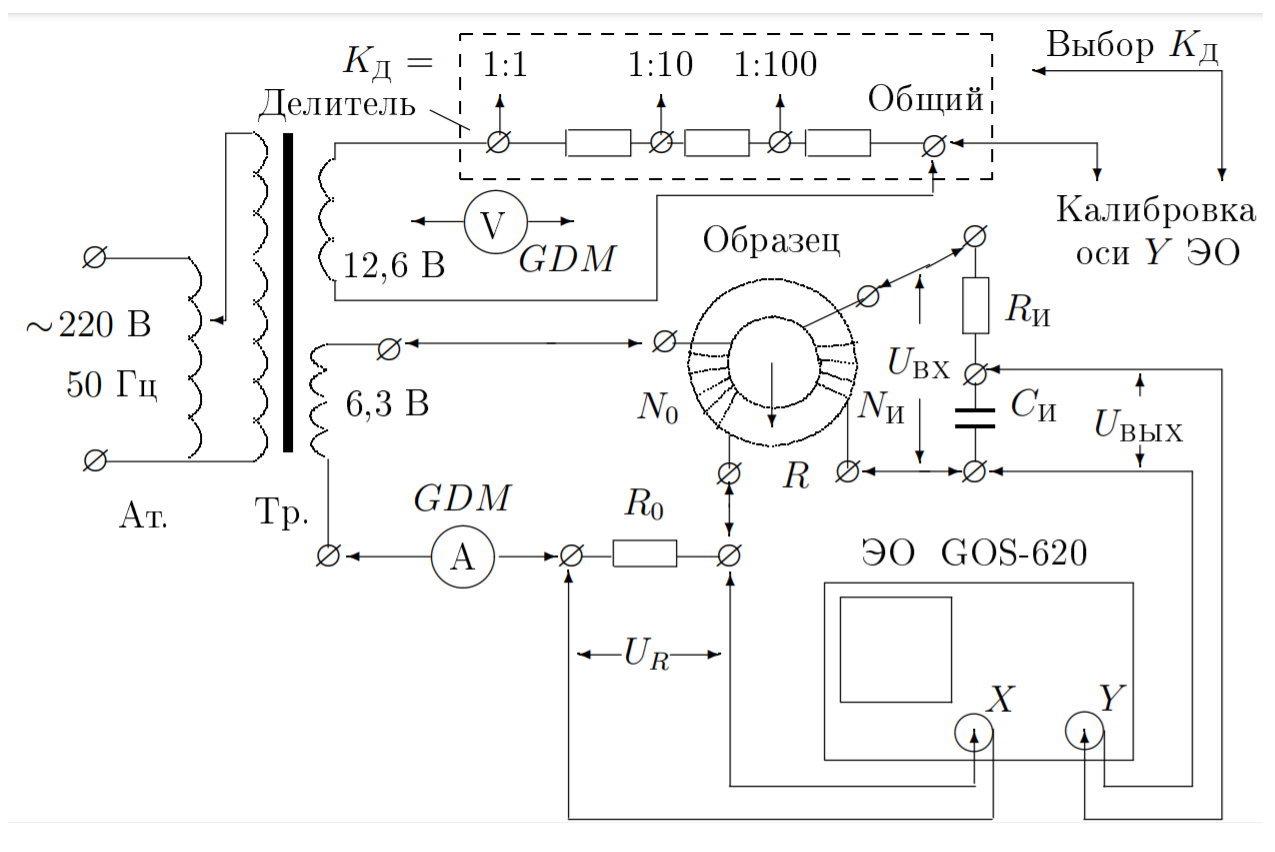
\includegraphics[scale=0.35]{img/device.png}
            \caption{Схема установки для исследования намагничивания образцов} \label{device}
        \end{figure}

        Действующее значение переменного тока в обмотке $N_0$ измеряется амперметром $A$ (мультиметром GDM). Последовательно с амперметром включено сопротивление $R_0$, напряжение с которого подаётся на вход $X$ электронного осциллографа (ЭО). Это напряжение пропорционально току в обмотке $N_0$, а следовательно и напряжённости $H$ магнитного поля в образце.

        Для измерения магнитной индукции $B$ с измерительной обмотки $N_{\text{и}}$ на вход интегрирующей $RC$-цепочки подаётся напряжение $U_{\text{и}}$ ($U_{\text{вх}}$), пропорциональное производной $\dot{B}$, а с выхода снимается напряжение $U_C$ ($U_{\text{вых}}$), пропорциональное величине $B$, и подаётся на вход $Y$ осциллографа.

        Замкнутая кривая, возникающая на экране, воспроизводит в некотором масштабе (различном для осей $X$ и $Y$) петлю гистерезиса. Чтобы придать этой кривой количественный смысл, необходимо установить масштабы изображения, т.е. провести калибровку каналов $X$ и $Y$ ЭО. Для этого, во-первых, надо узнать, каким напряжениям (или токам) соответствуют амплитуды сигналов, видимых на экране, и во-вторых, -- каким значениям $B$ и $H$ соответствуют эти напряжения (или токи).

        \textbf{Измерения напряжения с помощью осциллографа.} Исследуемый сигнал подаётся на вход $X$: длина $2x$ горизонтальной черты, наблюдаемой на экране, характеризует удвоенную амплитуду сигнала.

        Если известна чувствительность усилителя $K_X$ в вольтах на деление шкалы экрана, то удвоенная амплитуда напряжения определяется произведением\[2U_{X,0}=2x\cdot K_X.\]Напряжение, подаваемое на ось $Y$, измеряется аналогично.

        Калибровку осей осциллографа ($K_X$ и $K_Y$) можно использовать для построения кривой гистерезиса в координатах $B$ и $H$: зная величину сопротивления $R_0$, с которого снимается сигнал, можно определить чувствительность канала по току $K_{XI}=\frac{K_X}{R_0}\ \left[\frac{\text{А}}{\text{дел}}\right]$ и затем определить цену деления шкалы в $\frac{\text{А}}{\text{м}}$.

        Зная чувствительность $K_Y$, можно рассчитать цену деления вертикальной шкалы ЭО в теслах.

        Наличие в схеме амперметра и вольтметра позволяет провести \textit{независимую калибровку} усилителей ЭО, т.е. проверить значения коэффициентов $K_X$ и $K_Y$ (ручки регулировки усиления ЭО могут быть сбиты).

        \textbf{Проверка калибровки горизонтальной оси ЭО с помощью амперметра} проводится при закороченной обмотке $N_0$. Эта обмотка с помещённым в неё ферромагнитным образцом является нелинейным элементом, так что ток в ней не имеет синусоидальной формы, и это не позволяет связать амплитуду тока с показаниями амперметра.

        При закороченной обмотке $N_0$ амперметр $A$ измеряет эффективное значение синусоидального тока $I_{\text{эф}}$, текущего через известное сопротивление $R_0$. Сигнал с этого сопротивления подаётся на вход $X$ ЭО. Измерив $2x$ -- длину горизонтальной прямой на экране, можно рассчитать $m_X$ -- чувствительность канала $X$:\[m_X=\frac{2\sqrt2R_0I_{\text{эф}}}{2x}\quad\left[\frac{\text{В}}{\text{дел}}\right].\]

        \textbf{Проверка калибровки вертикальной оси ЭО с помощью вольтметра.} Сигнал с обмотки 12,6 В понижающего трансформатора (\ref{device}) подаётся на делитель напряжения. Часть этого напряжения снимается с делителя с коэффициентом деления $K_{\text{д}}$ ($\frac{1}{10}$ или $\frac{1}{100}$) и подаётся на вход $Y$ ЭО (вместо напряжения $U_C$). Мультиметр $V$ измеряет напряжение $U_{\text{эф}}$ на этих же клеммах делителя. Измерив $2y$ -- длину вертикальной прямой на экране, можно рассчитать чувствительность канала $Y$:\[m_Y=\frac{2\sqrt2R_0U_{\text{эф}}}{2x}\quad\left[\frac{\text{В}}{\text{дел}}\right].\]

        При этом тороид должен быть отключен, так как несинусоидальный ток нагрузки в первичной обмотке тороида приводит к искажению формы кривой напряжения и на обмотке трансформатора, питающей делитель.

        \textbf{Постоянную времени RC-цепочки} можно определить экспериментально. С обмотки 6,3 В на вход интегрирующей цепочки подаётся синусоидальное напряжения $U_{\text{вх}}$. На вход $Y$ осциллографа поочерёдно подаются сигналы со входа ($U_{\text{вх}}$) и выхода ($U_{\text{вых}}$) $RC$-цепочки. Измерив амплитуды этих сигналов с помощью осциллографа, можно рассчитать постоянную времени $\tau=RC$. Тогда\[RC=\frac{U_{\text{вх}}}{\Omega U_{\text{вых}}}.\]

    \section{Ход работы}

        \subsection{Проверка калибровки шкал осциллографа}

            Результат в таблице \ref{tab:calibr}

            \begin{table}[!ht]
                \centering
                \begin{tabular}{|c|c|c|c|}
                    \hline

                    \multicolumn{2}{|c|}{$K_x, \frac{мВ}{дел}$} & \multicolumn{2}{c|}{$K_y, \frac{мВ}{дел}$} \\ \hline
                    Осцилл. & Калибр. & Осцилл. & Калибр.\\ \hline
                    20 & 18.3 & 20 & 20.5\\ \hline
                    100 & 94 & 10 & 0.08\\ \hline

                \end{tabular}
                \caption{Результаты калибровки шкал осциллографа}
                \label{tab:calibr}
            \end{table}

        \subsection{Измерение параметров RC-ячейки}

            \begin{align*}
                \tau = \frac{U_{вх}}{U_{вых} \omega_0} = \frac{5.65~В}{0.042~В \cdot 2\pi50~Гц} &= 0.43~с
            \end{align*}

            \begin{align*}
                \tau = RC = 20~кОм \cdot 20~мкФ &= 0.4~с
            \end{align*}

            Как видим, результаты почти совпали. Также выполняется условие $R >> \frac{1}{\omega C}$ ($20000 >> 159$).

        \subsection{Обработка результатов}

            Графики и таблица итоговых результатов представлены ниже.

            \begin{figure}[!ht]
                \centering
                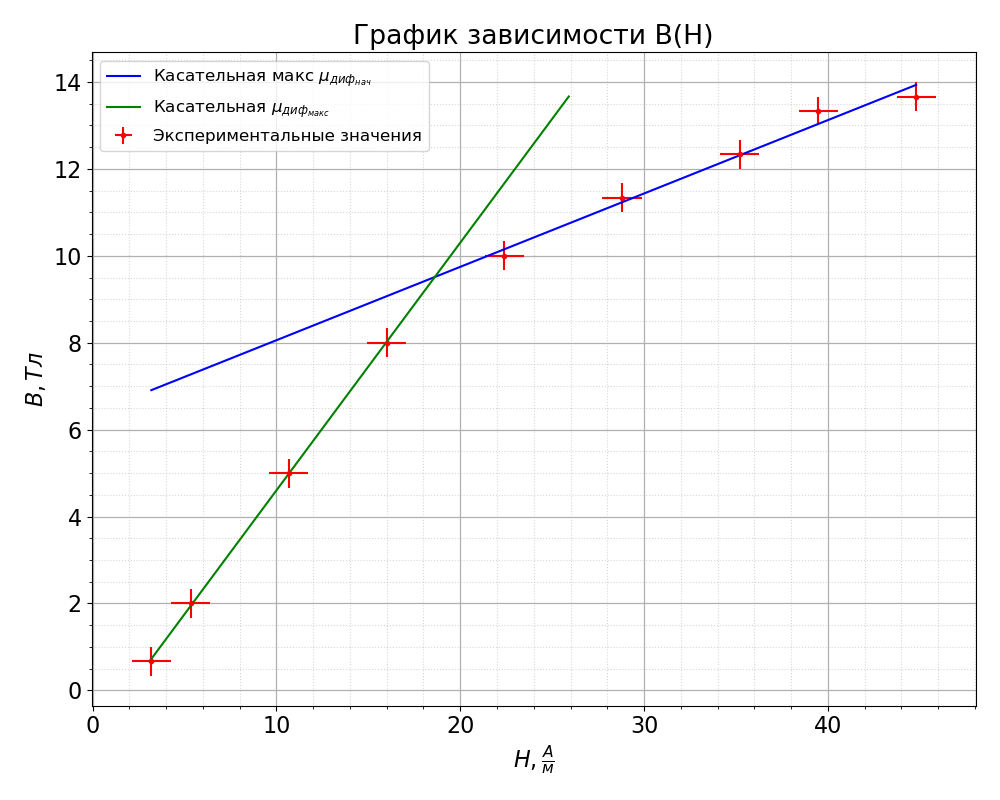
\includegraphics[width=0.65\textwidth]{img/plot_Fe.png}
                \caption{График зависимости $B(H)$ для феррита}
                \label{plot:Fe}
            \end{figure}

            \begin{figure}[!ht]
                \centering
                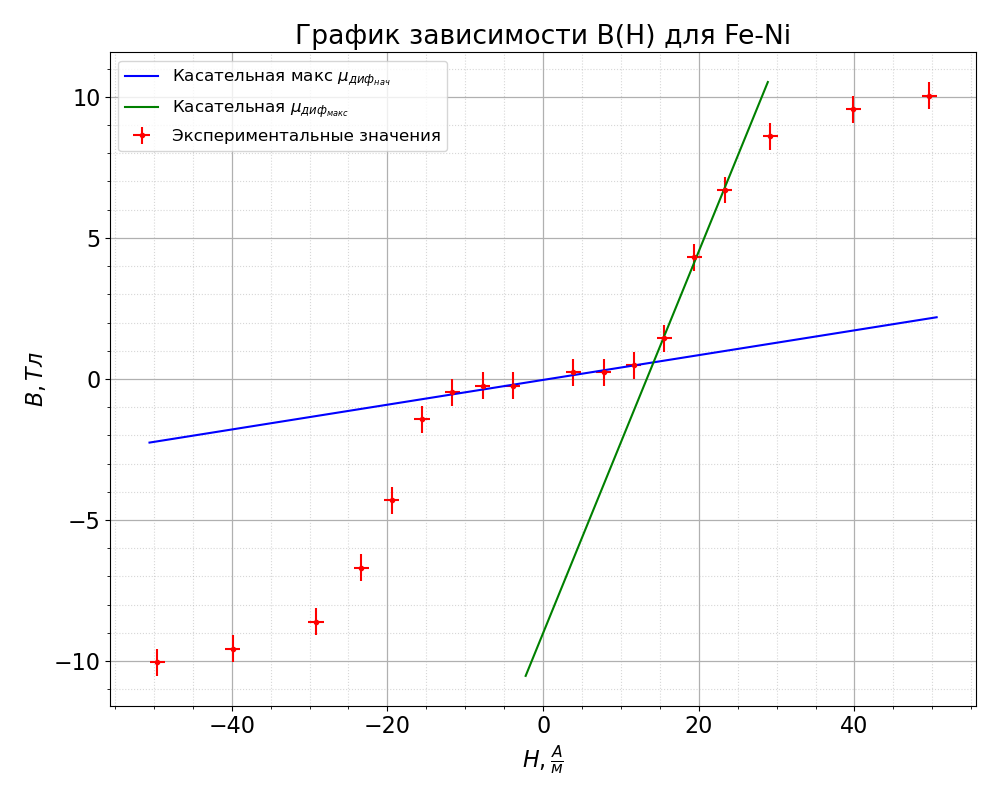
\includegraphics[width=0.65\textwidth]{img/plot_FeNi.png}
                \caption{График зависимости $B(H)$ для пермаллоя}
                \label{plot:FeNi}
            \end{figure}

            \begin{figure}[!ht]
                \centering
                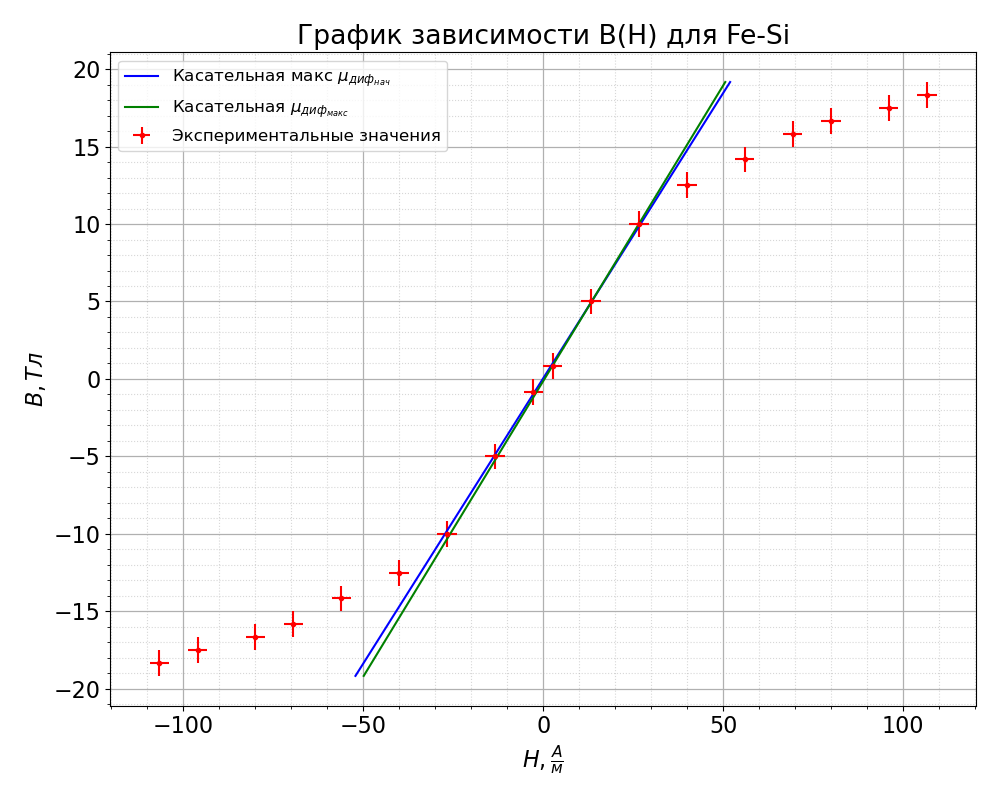
\includegraphics[width=0.65\textwidth]{img/plot_FeSi.png}
                \caption{График зависимости $B(H)$ для кремнистого железа}
                \label{plot:FeSi}
            \end{figure}

            \begin{table}[!ht]
                \centering
                \begin{tabular}{|c|c|c|c|}
                    \hline

                    Материал & Fe & Fe-Ni & Fe-Si\\ \hline
                    $I_{max}, мА$ & $160.00 \pm 0.01$ & $200.00 \pm 0.01$ & $800.00 \pm 0.01$\\ \hline
                    $K_x, \frac{В}{дел}$ & 0.02 & 0.02 & 0.02\\ \hline
                    $K_y, \frac{В}{дел}$ & 0.01 & 0.1 & 0.01\\ \hline
                    $H, \frac{А/м}{дел}$ & 10.7 & 9.7 & 26.7\\ \hline
                    $B, \frac{Тл}{дел}$ & 3.3 & 4.8 & 8.3\\ \hline
                    $H_{max}, А/м$ & $45 \pm 1$ & $49.58 \pm 0.97$ & $107 \pm 3$\\ \hline
                    $B_s, Тл$ & $13.7 \pm 0.3$ & $10.0 \pm 0.5$ & $18.3 \pm 0.8$\\ \hline
                    $H_c, А/м$ & $6 \pm 1$ & $5.83 \pm 0.97$ & $16 \pm 3$\\ \hline
                    $B_r, Тл$ & $5.3 \pm 0.3$ & $7.7 \pm 0.5$ & $13.3 \pm 0.8$\\ \hline
                    $\mu_{диф_{нач}}$ & $0.29 \pm 0.08$ & $0.04 \pm 0.02$ & $0.37 \pm 0.02$\\ \hline
                    $\mu_{диф_{макс}}$ & $0.58 \pm 0.01$ & $0.68 \pm 0.04$ & $0.382 \pm 0.004$\\ \hline

                \end{tabular}
                \caption{Результаты расчётов}
                \label{tab:res}
            \end{table}

    \section{Вывод}

        Изучили петли гистерезиса различных ферромагнитных материалов в переменных токах.

        Сравним полученные результаты с табличными значениями:

        \begin{table}[!ht]
            \centering
            \begin{tabular}{|c|c|c|c|c|}
                \hline
                & Ампл. & Fe-Ni & Fe-Si & Феррит \\ \hline
                эксп & \multirow{2}{*}{$H_c$, A/м} & $5.83 \pm 0.97$ & $16 \pm 3$ & $6 \pm 1$ \\ \cline{1-1} \cline{3-5}
                табл &  & 4 & 8 & 8 \\ \hline
                эксп & \multirow{2}{*}{$B_s$, Тл} & $10.0 \pm 0.5$ & $18.3 \pm 0.8$ & $13.7 \pm 0.3$ \\ \cline{1-1} \cline{3-5}
                табл &  & 1.1 & 2 & 0.2-0.4 \\ \hline
            \end{tabular}\\
            \caption{Результаты расчётов и табличные значения}
            \label{tab:tab_and_res}
        \end{table}

        Значения индукции насыщения достаточно сильно отличаются от табличных. Это можно объяснить неточностью определения момента, в который петля становится предельной.

        Проверки калибровки показала хороший результат.

        Измеренные параметры RC-ячейки почти совпали с указанными на установке.

\end{document}
